\chapter{Návrh dílčích bloků}
\label{kap:navrh-dilnich-bloku}
    Tato kapitola se důkladněji věnuje návrhu jednotlivých částí zařízení tak, aby splnily požadavky specifikované v sekci~\ref{sec:pozadavky}. Je zde vždy stručně rozebrána problematika týkající se daného modulu, popsán princip jeho funkce a následně popsána (TODO synonymum jiné) tvorba elektrického schématu spolu s výběrem vhodných komponent.

\section{Komunikační rozhraní}
\label{sec:komunikacni-rozhrani}
    Komunikační rozhraní mezi řídícím modulem a periferiemi není samo o~sobě funkčním modulem, ale je zde rozebráno jako první, protože právě od jeho specifikace se následně odvíjí tvorba zbytku zařízení. 

    Úkolem rozhraní je obousměrně komunikovat s~periferiemi, tedy např. stahovat data z~připojených sensorů a zároveň za pomoci přikazů periferie řídit. Kromě datové komunikace musí rozhraní periferie také napájet a to i v~případě energeticky náročnějších obvodů jako např. osvětlení. 
    
    \subsection{Výběr datové sběrnice}
        Existuje celá řada datových sběrnic, které jsou v~elektrotechnice hojně využívány. Každá z~nich má své výhody a nevýhody stejně jako jisté limitace použití. V~tab.~\ref{tab:porovnani-sbernic} se nachází výčet různých sběrnic, které byly při výběru uvažovány. 

        \begin{table}[h]
            \centering
            \caption{Datové sběrnice, porovnání~\cite{prodigy-spi-i2c}.}
            \label{tab:porovnani-sbernic}
            \begin{tabularx}{\textwidth}{|p{1.3cm}|X|X|X|}
            \hline
            \textbf{Typ} & \textbf{Výhody} & \textbf{Nevýhody} & \textbf{Limitace} \\
            \hline\hline
            SPI & 
            \begin{tabular}[t]{@{}p{4cm}@{}}
            - Více zařízení na sběrnici \\
            - Vysoká rychlost přenosu dat \\
            - Jednoduchý protokol \\
            \end{tabular} &
            \begin{tabular}[t]{@{}p{4cm}@{}}
            - Nutný CS pin pro každé zařízení \\
            \end{tabular} &
            \begin{tabular}[t]{@{}p{4cm}@{}}
            - Určeno na krátkou vzdálenost \\
            \end{tabular} \\
            \hline
            I\(^{2}\)C &
            \begin{tabular}[t]{@{}p{4cm}@{}}
            - Pouze 2 piny \\
            - Více zařízení -- 128 adres \\
            \end{tabular} &
            \begin{tabular}[t]{@{}p{4cm}@{}}
            - Riziko kolize adres \\
            - Nižší rychlost přenosu dat proti SPI \\
            \end{tabular} &
            \begin{tabular}[t]{@{}p{4cm}@{}}
            - Určeno na krátkou vzdálenost \\
            \end{tabular} \\
            \hline
            CAN &
            \begin{tabular}[t]{@{}p{4cm}@{}}
            - Vysoká spolehlivost \\
            - Dlouhé propojení \\
            \end{tabular} &
            \begin{tabular}[t]{@{}p{4cm}@{}}
            - Vyšší náklady na implementaci \\
            - Nižší rychlost přenosu dat \\
            \end{tabular} &
            \begin{tabular}[t]{@{}p{4cm}@{}}
            - Nepodporovano běžnými MCU -- nutný externí řadič \\
            \end{tabular} \\
            \hline
            UART &
            \begin{tabular}[t]{@{}p{4cm}@{}}
            - Jednoduchá implementace \\
            - Možnost asynchronní komunikace \\
            \end{tabular} &
            \begin{tabular}[t]{@{}p{4cm}@{}}
            - Nižší rychlost přenosu dat proti SPI \\
            - Pouze 2 zařízení \\
            \end{tabular} &
            \begin{tabular}[t]{@{}p{4cm}@{}}
            - Pouze 2 zařízení \\
            - Určeno na krátkou vzdálenost \\
            \end{tabular} \\
            \hline
            \end{tabularx}
            
        \end{table}






        Protože hlavní šasi zařízení nabízí dva konektory, ale žádoucí je připojit větší předem nedefinovaný počet periferií, je potřeba, aby sběrnice umožnila připojení více zařízení. 
        Obecný problém všech sběrnic je omezení jejich maximální délky, s~rostoucí délkou se sběrnice snáze zaruší, navíc z~důvodu parazitních vlastností vedení dochází k~zaoblení ostrých hran signálu, dlouhé vedení se chová jako filtr typu dolní propust. V~důsledku toho se snižuje maximální rychlost sběrnice.
        
        Sběrnice SPI nebo \acs{i2c} je obecně doporučeno používat pouze v~rámci DPS, tedy na krátké vzdálenosti. Při snížení rychlosti je možné je používat i na větší vzdálenost, ovšem modulární scénář vytvářeného systému teoreticky nestanovuje žádný délkový limit a bylo by velmi obtížné spolehlivě určit, kolik periferií uživatel může za sebe zapojit při zachování spolehlivé komunikace.

        UART je výhodný svou jednoduchou implementací a umožňuje obousměrnou asynchronní komunikaci. Nevýhodou je že funguje pouze pro dvě zařízení. Jednou z možností jak tuto limitaci obejít by bylo zavedení řetězového způsobu komunikace, kdy by každé zařízení komunikovalo se dvěmi sousedními a informace by se postupně předávala dále až k cílovému zařízení. Tento systém je relativně jednoduchý, ale například v případě poruchy jednoho zařízení se odpojí všechna následující zařízení, což může mít neočekávané následky.

        Sběrnice CAN je určena pro provoz v~průmyslovém prostředí (zejména je používána v~automobilovém průmyslu) a díky své robustnější konstrukci ji lze bez problému použít i na delší vzdálenosti a pro více zařízení. Při komunikaci je používán diferenční pár vodičů, takže i odolnost proti rušení je výrazně lepší. Nevýhodou je ale její o něco složitěkší a dražší implementace. Většina běžných mikrokontrolerů nemá pro CAN vestavěnou periferii a je tak potřeba buďto zvolit dražší mikrokontroler nebo připojit externí ovladač řízený např. přes SPI, dále je nutné přidat i řadič, který převede signál na diferenční pár a umožní také zvýšit provozní napětí na 12  nebo \qty{24}{V}, čímž dojde ještě k lepšímu potlačení šumu.

    \subsection{Sběrnice CAN}
        Po důkladné rešerši a zvážení zmíněných kladů a záporů byla  zvolena sběrnice CAN. ESP32 jakožto mikrokontroler řídící jednotky obsahuje vestavený CAN kontroler a pro moduly periferií byl na základě tohoto rozhodnutí zvolen také vhodný mikrokontroler. Co se týče nutnosti přidání řadiče, jedná se sice o další součástku, která na první pohled navyšuje cenu zařízení, kromě převodu signálu na diferenční pár ale zajišťuje také ochranu konektorů proti mnoha nežádoucím jevům jako je zkrat, ESD výboj nebo přepětí. Tímto se ve výsledku celé zapojení zlevní a zjednoduší.


   

\section{Řídící jednotka}
% \textit{TODO: shrnutí funkce a požadavků -- komunikace s periferiemi, napajeni, wifi, status - led + display} 
    Jedná se o~jádro celého zařízení. Její funkcí je řízení celého systému a zároveň komunikace s~uživatelem za pomoci Wi-Fi. Musí v~sobě nést informaci o~konfiguraci systému a na jejím základě zpracovávat data z~jednotlivých připojených periferií. Podle uživatelem nastavených scénářů pak dynamicky reaguje na změny hodnot měřených akvaristických veličin a ovládá akční členy (osvětlení, ohřev, filtr vody). Za pomoci displaye a LED pásku také informuje uživatele o~momentálním stavu zařízení. 

    Řídící jednotka bude tvořena jednou speciálně navrženou DPS, která kromě samotného mikrokontroleru bude obsahovat také obvody ke snížení napájecího napětí externího zdroje na hodnotu \qty{5.2}{V} (odůvodnění v~sekci~\ref{subsec:pocet-a-fce-vodicu-sbernice}). Toto napětí pak bude dále používáno pro napájení samotného mikrokontroleru řídící jednotky a zároveň vyvedeno na konektor pro připojení periferií. Blokové schéma na úrovni logických bloků v~rámci jedné DPS je na obr.~\ref{fig:ridici-jednotka-blokove-schema}, jednotlivým částem se blíže věnují další sekce. Celé schéma je k~dispozici v~příloze~\ref{priloha:schema-ridici-jednotka}.

    \begin{figure}[h!]
        \centering
        % trim=left bottom right top
        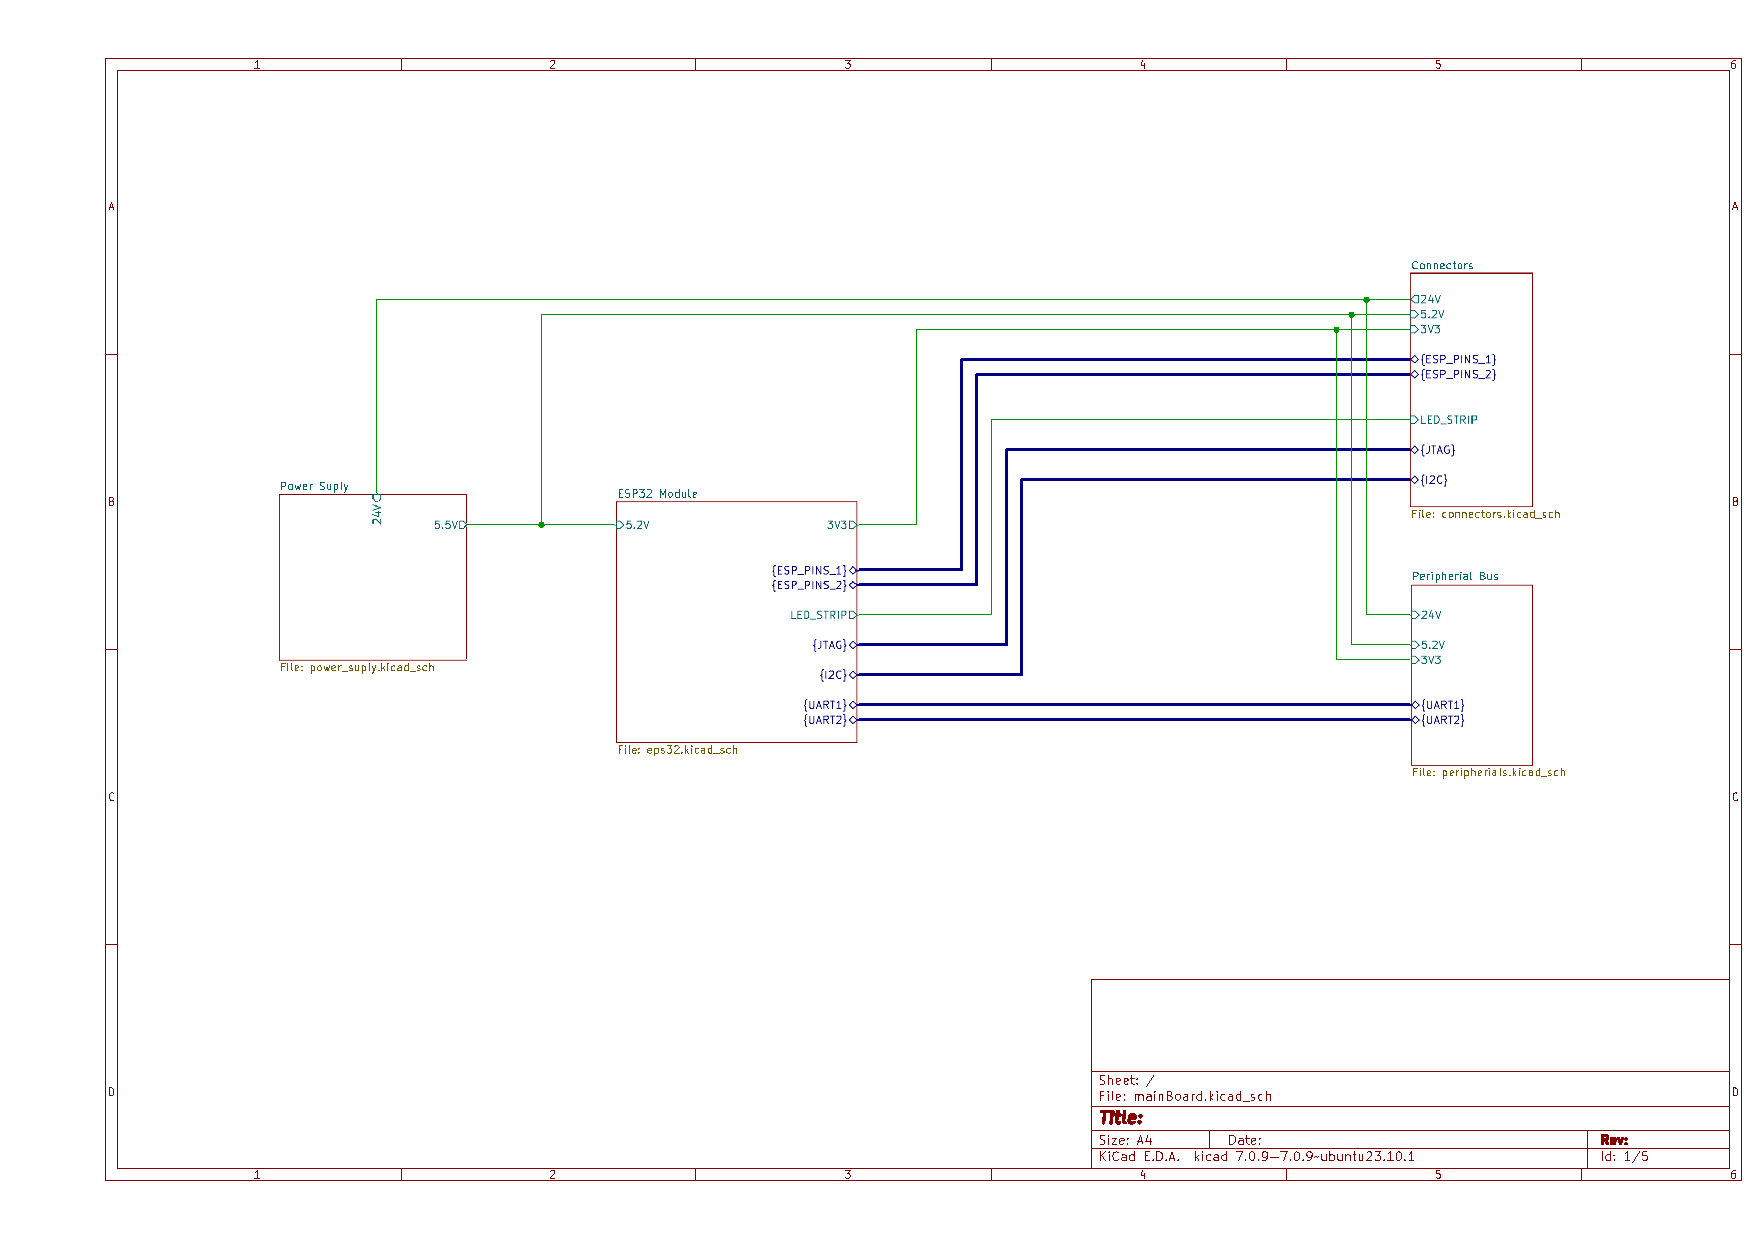
\includegraphics
        [
            width=\textwidth, 
            page=1, 
            trim=4.5cm 7.5cm 3cm 4cm, 
            clip
        ]{obrazky/exportovane/main-board-schematic.pdf}
        \caption{Blokové schéma řídící jednotky. Vytvořeno v~KiCad 7.0.}
        \label{fig:ridici-jednotka-blokove-schema}
    \end{figure}

    \subsection{MCU}
        % \textit{TODO: zdůvodnit výběr ESP32, informace o něm a schéma potřebných obvodů} 
        Při výběru vhodného mikrokontroleru bylo potřeba zohlednit výše zmíněné požadavky, tedy zejména Wi-Fi konektivitu a dostatečný výkon k~její obsluze, dvě volné UART periferie a dostatek GPIO pinů pro připojení zbylých modulů v~hlavním šasi (viz obr.~\ref{fig:blokove-schema}). Na trhu existuje vícero výrobců nabízejících mikrokontrolery s~vhodnými parametry, z~důvodu jednoduchosti použití a nízké ceny byl nakonec zvolen model ESP32 od firmy Espressif, konkrétně modul WROOM-32E~\cite{esp32-wroom-32e-datasheet} s~čipem ESP32-D0WDR2-V3~\cite{esp32-datasheet}. Tento modul je často využíván v~různých hobby projektech, ale také v~komerčních aplikacích zejména v~oblasti chytré domácnosti. Z~tohoto důvodu k~němu existuje velká škála softwarových knihoven a v~rámci komunity uživatelů je také sdíleno mnoho projektů, kterými je možné se inspirovat.

    \subsection{Zapojení ESP32 modulu}
        Při tvorbě schématu bylo vycházeno z~dokumentace výrobce~\cite{esp32-wroom-32e-datasheet} a také ze schématů různých existujících vývojových desek. K~zajištění správné a spolehlivé funkce modulu je potřeba dodržet několik věcí. Výřez schématu obsahující potřebné doplňující obvody je na obr.~\ref{fig:ridici-jednotka-esp-obvody}.

        \begin{figure}[h!]
            \centering
            % trim=left bottom right top
            \includegraphics
            [
                width=0.9\textwidth, 
                page=2, 
                trim=2.5cm 6cm 15.5cm 1.5cm, 
                clip
            ]{obrazky/exportovane/main-board-schematic.pdf}
            \caption{Podpůrné obvody pro modul ESP32-WROOM-E. Vytvořeno v~KiCad 7.0.}
            \label{fig:ridici-jednotka-esp-obvody}
        \end{figure}

        Na napájecí pin (3V3) je třeba přivést stabilní napětí a opatřit ho blokovacími kondenzátory (C1, C3). Ke snížení napětí z~původních \qty{5,2}{V} na požadovaných \qty{3,3}{V} je použit lineární regulátor TLV76133 (U4). 
        
        Dále je potřeba přivést kladné napětí na povolovací pin (EN), z~dokumentace vyplývá, že by mělo být přivedeno až po ustálení napájecí linky. Uvedený čas nutný ke stabilizaci je roven \(t_{STBL}=\qty{50}{\micro\second}\)~\cite{esp32-datasheet}. Požadované zpoždění zajistí RC článek (R1, C2) s~časovou konstantou \(\tau\):
        \begin{equation}
            \tau=R_{1}C_{2}=\qty{10}{\kilo\ohm}\cdot \qty{1}{\micro\farad}=\qty{10}{\milli\second}
        \end{equation} 
        Jak je vidět, byla zvolena dostatečná návrhová rezerva. 

        Pro možnost resetu zařízení a nahrání nového firmware byla doplněna také dvě tlačítka (SW1, SW2)


    \clearpage
    \subsection{Napájecí obvod}
        \label{sec:ridici-jendotka-napajeci-obvod}
        % \textit{TODO: schéma, výpočet hodnot součástek}
        Pro napájení celého zařízení bude použit externí zdroj stejnosměrného napětí \qty{24}{V}, toto napětí bude rozvedeno všem připojeným periferiím (viz sekce~\ref{subsec:pocet-a-fce-vodicu-sbernice}). Pro většinu komponent ale bude nutné napětí snížit, k~tomuto účelu bude využit DC/DC měnič typu buck s~požadovaným výstupním napětím \qty{5.2}{V}. Existuje celá řada čipů vyvinutých pro tento účel. Aplikace v~tomto zařízení je specifická svými požadavky na výstupní proud, zatímco samotná řídící jednotka nebude odebírat velký proud, není jasně dané, kolik periferí a s~jakými výkonovými požadavky uživatel k~systému připojí. Navržený měnič tak musí fungovat v~širším rozsahu proudů (řádově od desítek mA po jednotky A) a to s~co nejlepší účinností. 
        
        \begin{figure}[h!]
            \centering
            % trim=left bottom right top
            \includegraphics
            [
                width=0.9\textwidth, 
                page=3, 
                trim=5.5cm 4.5cm 4cm 2.5cm, 
                clip
            ]{obrazky/exportovane/main-board-schematic.pdf}
            \caption{Napájecí obvod řídící jednotky. Vytvořeno v~KiCad 7.0.}
            \label{fig:ridici-jednotka-napajeni}
        \end{figure}

        Po zvážení výše zmíněných požadavků byl jako základ buck měniče zvolen čip LM5148~\cite{lm5148-datasheet}, jedná se o~moderní součástku firmy Texas Instruments s~velkou výkonovou rezervou. Jelikož funguje pouze jako regulátor a je potřeba doplnit zapojení externími MOSFET tranzistory, většina tepelných ztrát vzniká právě na nich, čímž se sníží ohřev samotného čipu a zjednodušší chlazení. Na volbě tranzistorů závisí také výsledná účinnost měniče. Při návrhu zapojení této součástky byl použit nástroj Webench Power Designer~\cite{webench-power-designer}, který podle zadaných porametrů navrhne konkrétní schéma zapojení, provede simulaci a zobrazí grafy upravené na míru podle zvolených hodnot. Tento nástroj uvádí přibližnou účinnost zapojení jako \qty{88}{\percent}. V~navrženém schématu bylo posléze provedeno několik drobných změn, aby vše odpovídalo požadavkům uvedeným v~katalogovém listu součástky~\cite{lm5148-datasheet}. Výsledné zvolené zapojení se nachází na obr.~\ref{fig:ridici-jednotka-napajeni}. V~obrázku se nachází také odkazy ke konkrétním kapitolám katalogového listu relevantních k~volbě hodnot vybraných součástek. 

    \subsection{Ochrana konektorů}
        % \textit{TODO: popsat principy ochrany, schéma}
        Při návrhu elektronických obvodů je dobré myslet na různé problémy a poruchy, které by při provozu mohly nastat. Kromě snahy problémům předejít je důležité zařízení uzpůsobit pro maximální potlačení jejich následků. Důvodů k~ochraně navrhovaných obvodů je několik, na prvním místě by měla být vždy bezpečnost -- zařízení by při případné poruše např. nemělo způsobit požár, výbuch ani jinou podobnou situaci. Dalším důvodem je pak ochrana samotného zařízení a to zejména jeho drahých komponent. Přepětí na napájení nebo zkrat na konektoru nesmí mít za následek zničení procesoru popř. jiné dražší elektroniky~\cite{altium-circuit-protection}. 

        Citlivým místem z~hlediska ochrany jsou odkryté části zařízení, typicky uživateli přístupné konektory, v~případě zde popisovaného zařízení zejména konektory pro připojení periferií vyžadují při návrhu zvýšenou pozornost. Největším rizikem u~konektorů je elektrostatický výboj (ESD) při doteku uživatele popř. zkrat mezi jednotlivými vodiči při špatné manipulaci s~konektorem nebo doteku vodivým předmětem, v~případě zařízení pro akvaristiku není vyloučen ani kontakt s~vodou. 

        \begin{figure}[h!]
            \centering
            % trim=left bottom right top
            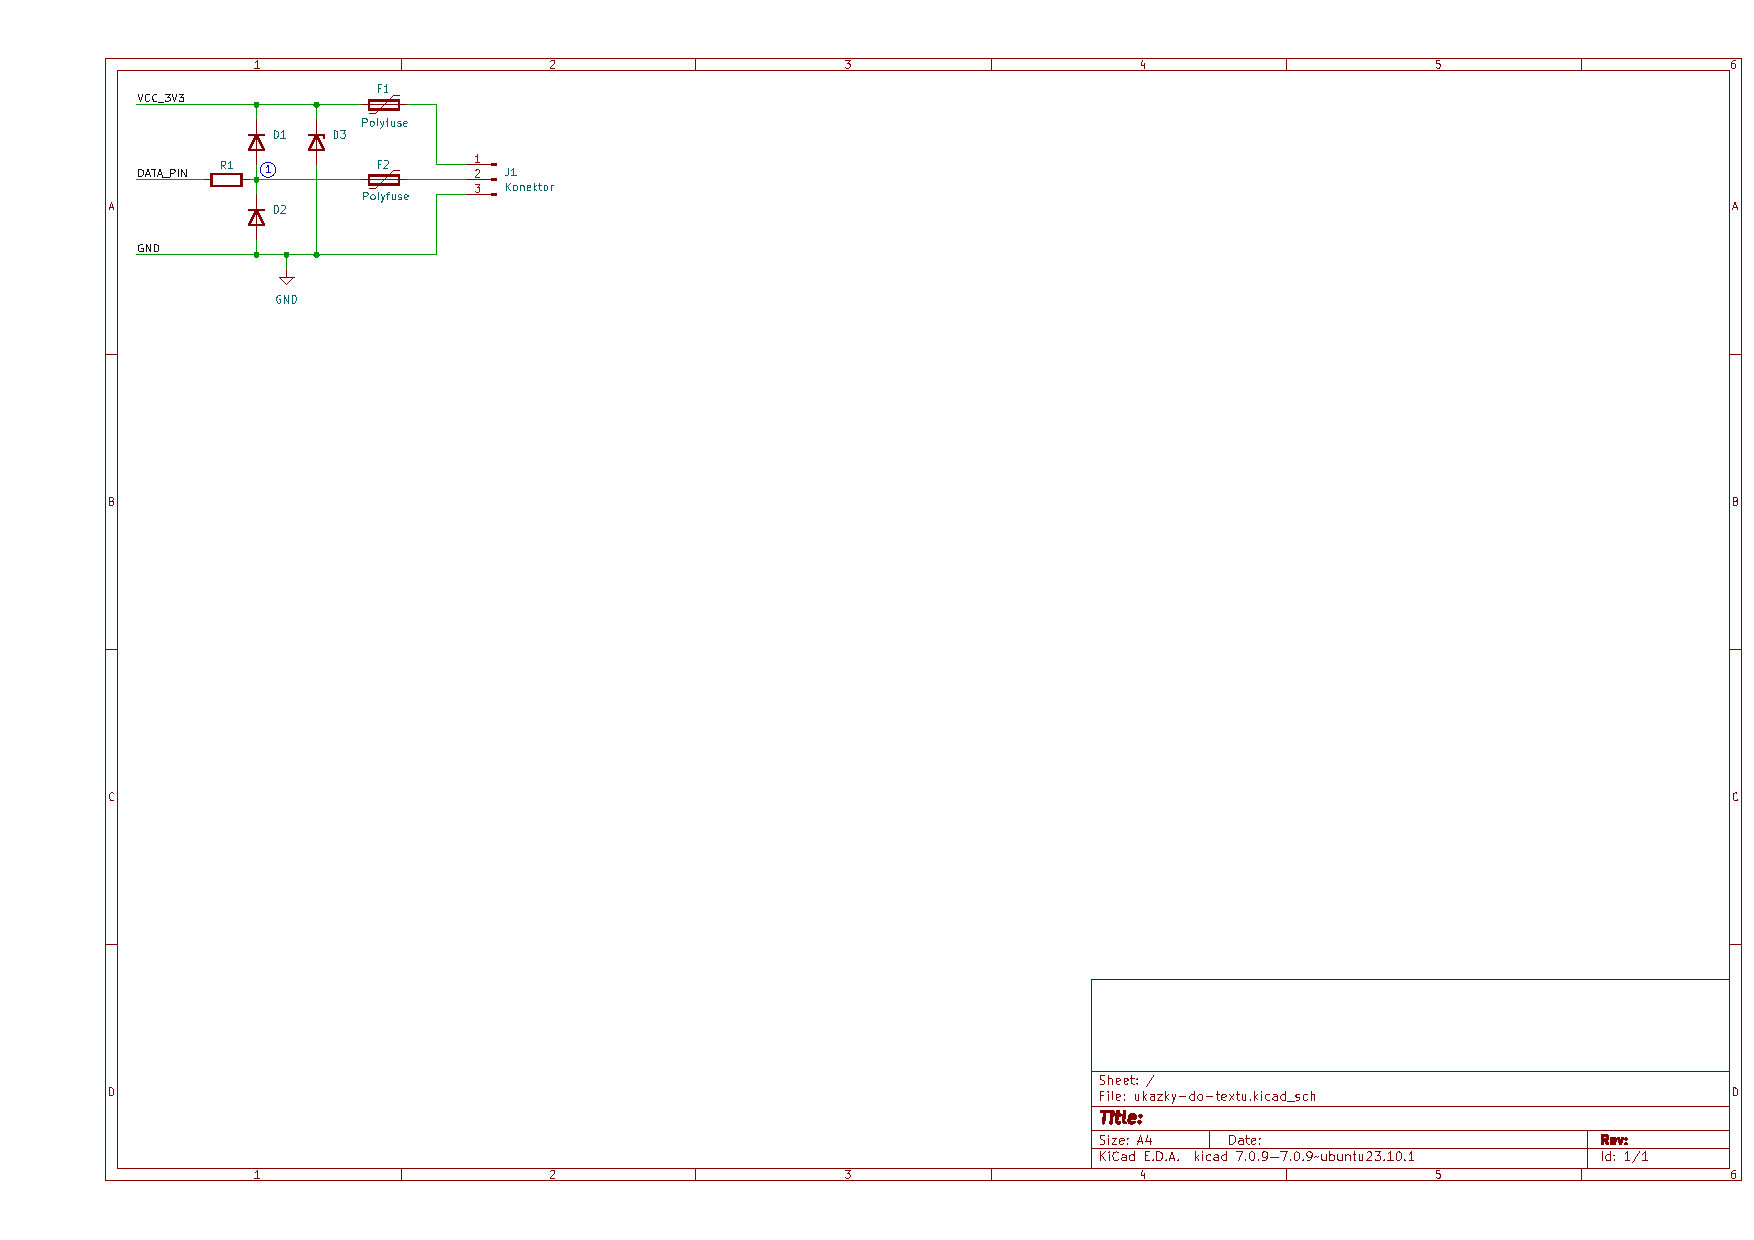
\includegraphics
            [
                width=0.9\textwidth, 
                page=1, 
                trim=2.1cm 16cm 20cm 1.3cm, 
                clip
            ]{obrazky/exportovane/ukazky-do-textu.pdf}
            \caption{Ochrana konektorů řídící jednotky, principiální schéma. Vytvořeno v~KiCad 7.0.}%
            \label{fig:ridici-jednotka-konektor-ochrana}
        \end{figure}

        \subsubsection{Princip zvolené ochrany}
        Na obr.~\ref{fig:ridici-jednotka-konektor-ochrana} je znárorněn princip použité ochrany proti přepětí na datové lince. Toto zapojení je účinné jako proti ESD, tak i proti zkratu~\cite{altium-esd-protection}. Je tvořeno několika stupni. Předmětem ochrany je zejména datový pin mikrokontroleru (na obr. jako DATA\_PIN). V~případě ESP32 je povolený rozsah napětí na datovém pinu \qty{-0.3}{V} až \qty{3.6}{V} a maximální přípustný vstupní proud \qty{28}{mA}, viz tab.~\ref{tab:esp32-elektricke-parametry}.

        Pokud se na pinu 2 konektoru (J1) objeví vyšší napětí, než je hodnota \(V_{CC} +V_{f} \), kdy \(V_{f} \) je prahové napětí diody (D1, resp. D2), stane se dioda (D1) propustnou, napětí se dále nezvyšuje a přebytečný proud je skrze tuto diodu odveden do napájecí větve (VCC\_3V3), obdobné chování pro záporné napětí zajistí dioda D2. Pokud by napájecí větev nebyla schopná přebytečný proud odvést a hrozil by na ní nárust napětí, dojde k~ovevření stabilizační Zenerovy diody (D3) a disipaci energie v~podobě tepla. Aby nedošlo k~trvalému tepelnému poškození diod, je v~obvodu zařazena vratná pojistka (ang. polyfuse, PPTC; ve schématu konkrétně F2). Při překročení povoleného proudu se pojistka zahřeje a v~návaznosti na to výrazně zvýší svůj odpor, čímž proud stabilizuje na pevně danou úroveň.

        Pro případ zkratu na napájení je přidána ještě jedna vratná pojistka (F1), která limituje proud napájecí větve na bezpečnou úroveň.

        Ve skutečném schématu (viz příloha~\ref{priloha:schema-ridici-jednotka-periferie}) jsou diody nahrazeny ekvivalentním integrovaným obvodem.

        \begin{table}[h]
            \centering
            \caption{Elektrické parametry ESP32, výňatek z~\cite{esp32-wroom-32e-datasheet}, platné pro \(V_{DD} =\qty{3,3}{V}\).}
            \label{tab:esp32-elektricke-parametry}
            \begin{tabular}{|l|l|l|l|l|}
            \hline
            \textbf{Parametr} & \textbf{Popis} & \textbf{Min} & \textbf{Typ} & \textbf{Max} \\ \hline\hline
            \(V_{IH}\) (V)   & High-level input voltage   & 2,475  & --  & 3,6          \\ \hline
            \(V_{IL}\) (V)   & Low-level input voltage    & -0,3 & --   & 0,825   \\ \hline
            \(I_{IH}\) (nA)  & High-level input current   & --   & --   & 50           \\ \hline
            \(I_{IL}\) (nA)  & Low-level input current    & --   & --   & 50           \\ \hline
            \(I_{OH}\) (mA)  & High-level source current  & --   & 40   & --           \\ \hline
            \(I_{OL}\) (mA)  & Low-level sink current     & --   & 28   & --           \\ \hline
            \end{tabular}
        \end{table}

        \newpage
        \subsubsection{Výpočet hodnot součástek}
            Při použití diody s~\(V_{f} =\qty{0.7}{V}\) je maximální napětí v~uzlu \circled{1} rovno:
            \begin{equation}
                V_{1} =V_{CC} +V_{f} = \num{3,3}+\num{0,7}=\qty{4}{V}
            \end{equation}
            Pro omezení proudu do pinu mikrokontroleru je do linky zařazen sériový rezistor (R1). Počítejme s~napětím na pinu rovnému \(V_{pin} =\qty{3.3}{V}\) a maximálnímu přípustnému proudu \(I_{OL} =\qty{28}{mA}\). Minimální hodnota odporu rezistoru se pak stanoví následujícím způsobem:
            \begin{equation}
                R_{1} =\frac{V_{1}- V_{pin}}{I_{OL} }=\frac{\num{4}-\num{3.3}}{\num{28e-3}}=\qty{25}{\ohm}
            \end{equation}

            Je možné zvolit také větší hodnotu odporu a z~hlediska ochrany si tak zajistit jistou návrhovou rezervu, příliš velká hodnota by však způsobila zhoršení přenosové rychlosti sběrnice. Pokud by ale došlo k~opačnému problému a to ke zkratování výstupu z~pinu se zemí (GND), byl by při hodnotě \qty{25}{\ohm} překročen maximální povolený výstupní proud z~pinu (\(I_{OH}=\qty{40}{mA}\)). Hodnota odporu z~hlediska takového zkratu by tedy musela být minimálně:
            \begin{equation}
                R_{1} =\frac{V_{pin}}{I_{OH} }=\frac{\num{3.3}}{\num{40e-3}}=\qty{82.5}{\ohm}
            \end{equation}
            Pro účely této práce byla zvolena hodnota sériových odporů \qty{100}{\ohm}, která splňuje všechny výše uvedené podmínky.

            Dále bylo nutné vybrat vratnou pojistku s~vhodnými parametry. Maximální provozní proud, který může po sběrnici téct je limitovaný sériovým odporem a pro zvolenou hodnotu \qty{100}{\ohm} odpovídá \(I_{max} =\qty{33}{mA}\), této hodnoty ale nikdy nedosáhne stabilně nýbrž pouze na krátký čas při změně mezi logickou nulou a jedničkou. Byla proto zvolena pojistka s~hodnotou limitního proudu \(I_{trip} =\qty{60}{mA}\) a běžného provozního proudu \(I_{hold} =\qty{20}{mA}\). 

            

            
\section{Ovládání 230V periferií}
\label{sec:perif-230v}
Jak vyplývá z~požadavků zařízení a přehledu používané akvaristické techniky, pro automatizovaný provoz akvária je nutné umožnit řídicí jednotce ovládat několik okruhů se síťovým napětím a spínat tak zvlášť zakoupené hotové spotřebiče pracující s~tímto napětím. Jedná se typicky o~ohřev vody, filtraci, popř. některé druhy osvětlení. 

\begin{figure}[h!]
    \centering
    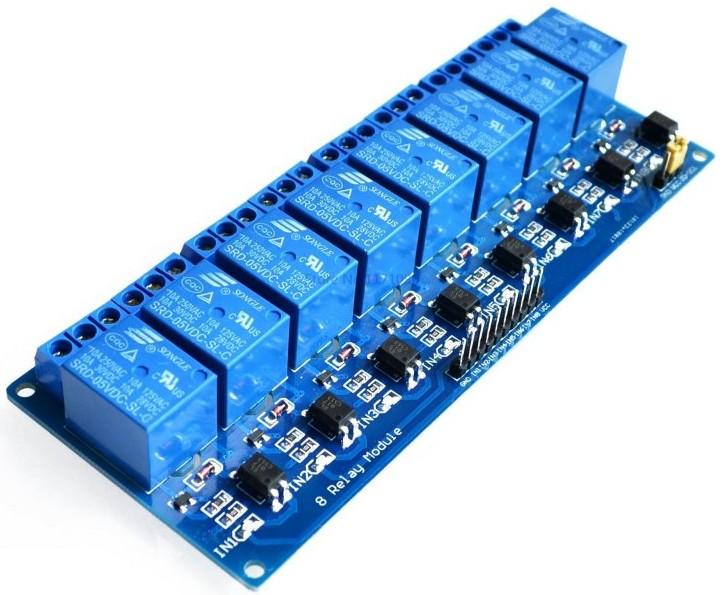
\includegraphics[width=0.6\textwidth]{obrazky/230/rele.jpg}
    \caption{TODO vyměnit: Relé modul, ilustrační foto. Převzato z~\cite{eshop-laskakit-rele}.}
    \label{fig:obrazky-230-rele-jpg}
\end{figure}


Aby uživatel mohl spínaná zařízení bezpěčně připojit bez nutnosti odborné způsobilosti, nachází se na hlavním šasi zařízení čtyři standartní zásuvky (typ E) s~jednofázovým napětím \qty{230}{V}. Fázové vodiče jsou uvnitř zařízení přerušeny spínacími relé. Je použit předpřipravený modul disponující osmi relé~\cite{eshop-laskakit-rele}, čtyři z nich tedy zůstanou nevyužité a slouží jako rezerva pro případ poškození některého z~používaných relé nebo při potřebě budoucího rozšíření o~další zásuvky. 

Z~důvodu nedostatku pinů na mikrokontroléru řídicí jednotky (ESP32) je k~relé modulu připojen ještě jeden externí modul a to expandér \acs{gpio} pinů komunikující přes sběrnici \acs{i2c}~\cite{eshop-laskakit-expander}. Z~pohledu mikrokontroléru jsou tak všechny zásuvky ovládány pomocí dvou \acs{gpio} pinů (\acs{sda}, \acs{scl}), které je navíc možné dále využít pro připojení jiných periferií jako např. O\acs{led} displaje pro zobrazení stavu zařízení.

Relé na použitém modulu potřebuje pro spolehlivé sepnutí napětí alespoň \qty{5}{V}, logické signály řídicí jednotky ale pracují s napětím pouze \qty{3.3}{V}. Ze schématu na obr.~\ref{fig:relay-board-simp-schema} je vidět, že použitý relé modul je spínán signálem logické nuly, tímto způsobem je problém s rozdílnou úrovní napájení elegantně vyřešen. 

\begin{figure}[h!]
    \centering
    % trim=left bottom right top
    \includegraphics
    [
        width=\textwidth, 
        page=3, 
        trim=2.5cm 14.5cm 18cm 1.5cm, 
        clip
    ]{obrazky/exportovane/ukazky-do-textu.pdf}
    \caption{Schéma jednoho kanálu relé modulu. Vytvořeno v~KiCad 7.0.}
    \label{fig:relay-board-simp-schema}
\end{figure}

Do budoucna by bylo možným zlepšením a rozšířením této práce zahrnutí obou zmíněných modulů přímo na \acs{dps} řídicí jednotky. 
\section{Obecný modul periferie}
    % \textit{    TODO: vybrán MCU PIC16F15325 -- jednoduché zapojení + znám použití ze školy, cenově vychází nejlépe, když zohledníme požadavky na periferie (2x UART, PWM). } 

    % \textit{
    %     Moje představa je navrhnout jednoduchou univerzální desku, která bude mít PICku, LDO a napojené vstupní a výstupní UARTy + ochrany na výstupech, k ní budou pin headery a možnost vložit shield/dauther board, který bude mít případnou další elektroniku k obsluze senzoru atd. Když nebudu stíhat, což určitě nebudu :), tak může být třeba na prototypové desce, což bude asi rozumnější než objednávat 10 různých DPS a pak v každé řešit chyby.} 

    Díky zvolené koncepci systému je možné za periferii považovat jakékoliv zařízení schopné obousměrně komunikovat po navržené sběrnici. Není vyloučeno, aby byla každá periferie navržena zcela odlišně na základě svých vlastních požadavků na výkon, počet pinů nebo dostupná rozhraní daného MCU. Hlavní výhodou této koncepce je to, že periferie mohou být vyvíjeny postupně a přidávány do již funkčního a odladěného systému bez nutnosti modifikovat stávájící hardware. V případě chyby v návrhu periferie je také oprava méně náročná, než by tomu bylo v případě zabudování veškeré funkcionality přímo do řídící jednotky. 

    Nicméně pokud by byl pro každou periferii zvolen zcela jiný mikrokontroler a vytvořen vlastní návrh DPS, vývoj více periferií by byl zbytečně drahý a časově náročný. Proto byl zvolen koncept \uv{obecného modulu periferie}, tedy jedné DPS s konkrétním mikrokontrolerem zajišťující připojení k oběma stranám komunikačního rozhraní, napájení periferie a rozhraní pro programování. Kromě toho budou na DPS dvě dutinkové lišty, do kterých bude možné vsadit druhou DPS (popř. během vývoje pouze prototypovací desku) ve funkci dceřinné desky (ang. daughterboard). Vložená deska pak bude obsahovat obvody nutné přímo pro danou konkrétní periferii, např. pro teploměr to bude elektronika umožňující připojení teplotního čidla k mikrokontroleru. 

    V aktuální fázi tento práce byl pouze zvolen vyhovující mikrokontroler, návrh konkrétního schématu a rozložení DPS bude předmětem práce budoucí. 
    
    \subsection{MCU}

        Kritéria pro výběr mikrokontroleru byla následující:
        \begin{itemize}
            \item Musí nutně splňovat:
            \begin{itemize}
                \item 2x UART periferie -- pro komunikaci po sběrnici 
                \item PWM výstup -- řízení LED, popř. jiné
                \item Nízká cena 
            \end{itemize}
            \item Je výhodou:
            \begin{itemize}
                \item Dobrá dokumentace, komunita uživatelů
                \item Zkušenost autora s danou platformou
                \item Další periferie (I\(^2\)C, SPI, ...)
            \end{itemize}
        \end{itemize}

        Na základě těchto kritérií byl vybrán mikrokontroler \textbf{PIC16F15325} od firmy Microchip, ten splňuje všechna kritéria a disponuje také množstvím dalších periferií, které by mohly být v budoucnu užitečné~\cite{PIC16F15325}. 


% Zatím drbnu sem, ať zas pak nemusím mazat soubory


    % Přenecháno do BP :)

    % \section{Konkrétní periferie}
    %     \textit{TODO: stačí se jim věnovat až v BP a nebo je to porušení zadání, které způsobí rozložení studia? :) Jen ať vím, jak moc a na čem musím zabrat.}  



